%%%%%%%%%%%%%%%%%%%%%%%%%%%%%%%%%%%%%%%%%
% Thin Sectioned Essay
% LaTeX Template
% Version 1.0 (3/8/13)
%
% This template has been downloaded from:
% http://www.LaTeXTemplates.com
%
% Original Author:
% Nicolas Diaz (nsdiaz@uc.cl) with extensive modifications by:
% Vel (vel@latextemplates.com)
%
% License:
% CC BY-NC-SA 3.0 (http://creativecommons.org/licenses/by-nc-sa/3.0/)
%
%%%%%%%%%%%%%%%%%%%%%%%%%%%%%%%%%%%%%%%%%

%----------------------------------------------------------------------------------------
%	PACKAGES AND OTHER DOCUMENT CONFIGURATIONS
%----------------------------------------------------------------------------------------

\documentclass[a4paper, 11pt]{article} % Font size (can be 10pt, 11pt or 12pt) and paper size (remove a4paper for US letter paper)
%\usepackage[ngerman]{babel}
\usepackage[protrusion=true,expansion=true]{microtype} % Better typography
\usepackage{graphicx} % Required for including pictures
\usepackage{wrapfig} % Allows in-line images
\usepackage{blindtext}
\usepackage{mathpazo} % Use the Palatino font
\usepackage[T1]{fontenc} % Required for accented characters
\linespread{1.05} % Change line spacing here, Palatino benefits from a slight increase by default
% BibLaTex und Biber------------------------------------------------------------
\usepackage[
backend=biber,
style=numeric-comp,
%sortlocale=de_DE,
natbib=true,
hyperref=true,
url=true, 
doi=true,
eprint=false
]{biblatex}
\addbibresource{literature.bib}
% Biblatex Kompatibilität
\usepackage{csquotes}       
%%%%%%%%%%%%%%%%
\usepackage{tcolorbox}
\usepackage{hyperref}
\usepackage{amsmath}


%\setlength\bibitemsep{2\itemsep}	% increase space between entries by 0.5

%\DefineBibliographyStrings{ngerman}{ %et al anstelle von u.a.
%	andothers


\makeatletter
%\renewcommand\@biblabel[1]{\textbf{#1.}} % Change the square brackets for each bibliography item from '[1]' to '1.'
\renewcommand{\@listI}{\itemsep=0pt} % Reduce the space between items in the itemize and enumerate environments and the bibliography

\renewcommand{\maketitle}{ % Customize the title - do not edit title and author name here, see the TITLE block below
\begin{flushright} % Right align
{\LARGE\@title} % Increase the font size of the title

\vspace{50pt} % Some vertical space between the title and author name

{\large\@author} % Author name
\\\@date % Date

\vspace{40pt} % Some vertical space between the author block and abstract
\end{flushright}
}

%----------------------------------------------------------------------------------------
%	TITLE
%----------------------------------------------------------------------------------------

\title{\textbf{Comparison of SIFT and SURF algorithms: Speed and complexity vs. preciseness and robustness}\\ % Title
A computer vision essay} % Subtitle

\author{\textsc{Juri Fedjaev} % Author
\\{\textit{Technische Universit\"at M\"unchen}}} % Institution

\date{\today} % Date

%----------------------------------------------------------------------------------------

\begin{document}

\maketitle % Print the title section

%----------------------------------------------------------------------------------------
%	ABSTRACT AND KEYWORDS
%----------------------------------------------------------------------------------------

%\renewcommand{\abstractname}{Summary} % Uncomment to change the name of the abstract to something else

\begin{abstract}
This essay analyzes two state-of-the-art algorithms (SIFT and SURF) for feature detection and description regarding speed, complexity, preciseness and robustness. Each algorithm is first briefly revised. Subsequently, the inherent properties of the algorithms are analyzed and compared to each other. The SURF algorithm is theoretically more efficient and computationally less complex than SIFT, while still yielding comparable performance in terms of quality of the matches in many cases. However, SIFT is in general the more accurate algorithm, being less affected by disturbances such as image rotations, scaling or blurring. Surprisingly, however, SIFT quite often even outperforms SURF in practical applications in terms of speed due to more efficient implementations in available computer vision libraries.

\end{abstract}

\hspace*{3,6mm}\textit{Keywords:} SIFT , SURF , preciseness , complexity, robustness, speed % Keywords

\vspace{30pt} % Some vertical space between the abstract and first section

%----------------------------------------------------------------------------------------
%	ESSAY BODY
%----------------------------------------------------------------------------------------
\section{Introduction}
\label{sec:introduction}
Image feature detectors and descriptors need to be both fast and accurate at the same time. This requirement forms a major challenge in numerous computer vision tasks, such as object recognition or panoramic stitching. Other than that mentioned applications, scenarios involving real-time embedded systems (e.g. autonomous robot or vehicle navigation) require high performance algorithms that minimize the use of computational resources \cite{awad2016image}. \\
An object in a natural image comprises so-called \textit{interesting points}. Those interesting points may be extracted in order to describe the object, forming a \textit{feature descriptor}. By using this descriptor (extracted from training images), it is possible to exactly identify and locate that same object in a different image containing all sorts of other objects. In real world problems, different images of objects or landscapes are taken under changes of image scale, illumination and brightness, noise, and different views (e.g rotation). Therefore, it is important to extract features that are invariant to those disturbances in order to reliably perform object recognition \cite{juan2009comparison}.\\
Although many feature detection algorithms for reliable descriptors have been proposed in computer vision literature, they all have their own application domain. SIFT and SURF show both comparable performance in contemporary applications. SIFT is the better choice for practical, non-time critical applications. However, SURF remains a superior algorithm theoretically, in my opinion.\\
In this essay, SIFT and SURF algorithms are going to be compared in terms of their speed, complexity, preciseness and robustness. For that purpose, the algorithms will first be briefly revised in section~\ref{sec:revision}. In section~\ref{sec:comparison} the algorithms will then be compared in depth. The essay is concluded in section~\ref{sec:conclusion}.


%------------------------------------------------

\section{Revision of SIFT and SURF algorithms}
\label{sec:revision}
\subsection{Scale Invariant Feature Transform (SIFT)}
The SIFT \textit{(scale-invariant feature transform)} algorithm may be divided into four major stages of computation:
\begin{enumerate}
	\item \textbf{Scale-space extrema detection},
	\item \textbf{keypoint localization},
	\item \textbf{orientation assignment}, and 
	\item the computation of the \textbf{keypoint descriptor} \cite{lowe2004distinctive}. 
\end{enumerate}
The main difference to SURF lies in the very first part, the scale-space extrema detection. While both algorithms search for stable features, SIFT uses a cascade filtering approach by subsequently convolving the image with the difference-of-Gaussian (DoG) function. A multiplicative factor $k$ separates two nearby scales in the scale-space: 
\begin{align}
D(x,y,\sigma) = (G(x,y,k \sigma) - G(x,y,\sigma)) * I(x,y) = L(x,y,k \sigma) - L(x,y,\sigma).
\end{align}
These convolutions are applied in every octave of the scale-space. Subsequently, the filtered image $D(x,y,\sigma)$ is subsampled by a factor of $2$, forming a DoG-pyramid. As the image resolution is cut in half each iteration, the computational complexity decreases with higher levels in the pyramid. For extrema detection in $D(x,y,\sigma)$, each sample point is compared with its $26$ neighbors in $3\times3$ regions in adjoining scales \textit{(see figure~\ref{fig:neighbors})}. 
\begin{figure}
	\centering
	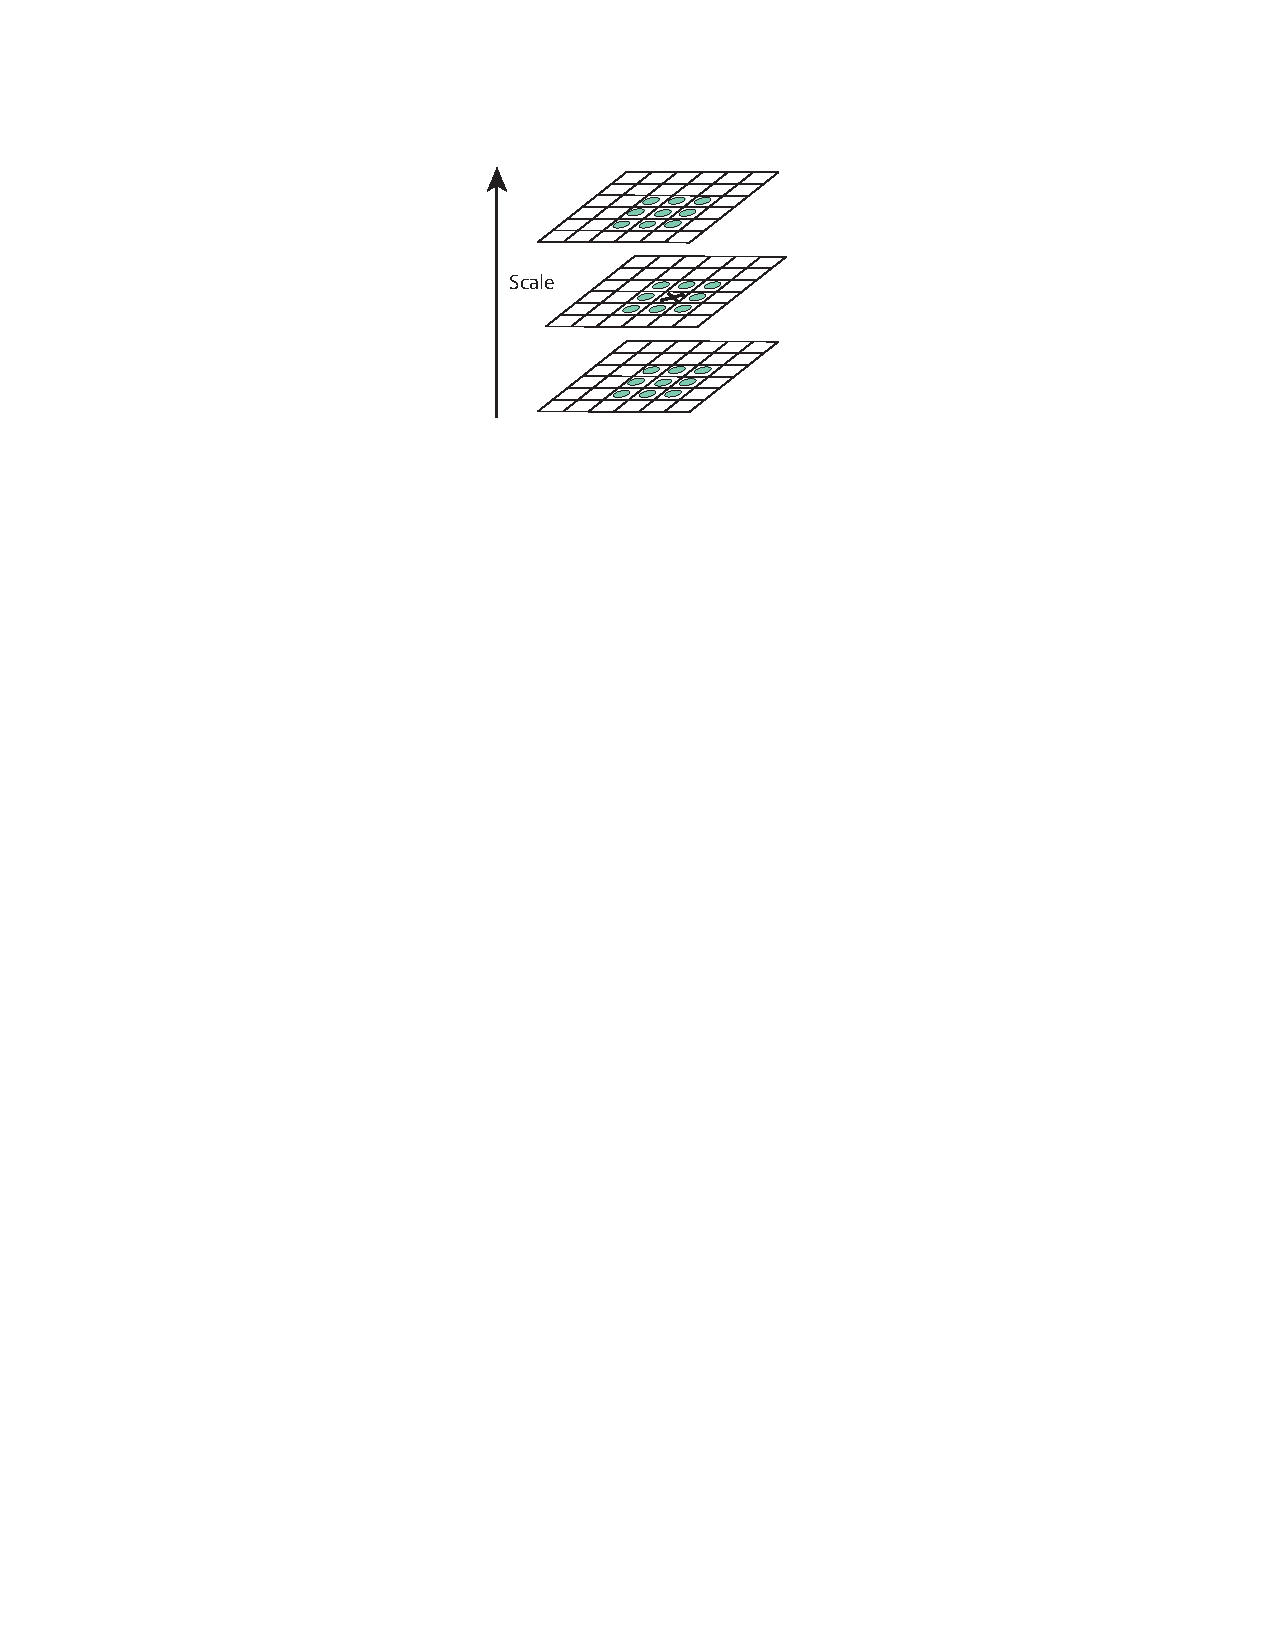
\includegraphics[width=0.4\textwidth]{images/neighbors}
	\caption{Extrema detection in the DoG images: each sample is compared to its 26 neighbors in the current and adjoining scales \cite{lowe2004distinctive}.}
	\label{fig:neighbors}
\end{figure}
After having found possible candidates and their exact location, unstable samples are filtered out. Low-contrast samples are detected by using the Taylor series approximation:
\begin{align}
D(\widetilde{x}) = D + \frac{1}{2} \frac{dD^T}{dx} \widetilde{x}
\end{align}
Every sample with a value of $|D(\widetilde{x})|$ less than 0.03 is discarded.\\
Further unstable samples are excluded by computing the trace of the Harris matrix $H$ of $D$. The standard value for $r$ used by \citeauthor{lowe2004distinctive} is $r = 10$.
\begin{align}
\frac{Tr(H)^2}{Det(H)} < \frac{(r+1)^2}{r}.
\end{align}
In a last step, the \textit{keypoint descriptor} is calculated. Therefore, the orientation (gradient) of each data sample needs to be determined:
\begin{align}
m(x,y) &= \sqrt{[L(x+1,y) -L(x-1,y)]^2 + [L(x,y+1) - L(x,y-1)]^2 }\\
\theta(x,y) &= tan^{-1}\left(\frac{L(x,y+1) - L(x,y-1)}{L(x+1,y) - L(x-1,y)} \right)
\end{align}
Finally, the gradients are weighted by a Gaussian function over $4 \times 4$ regions, accumulated into histograms and normalized, forming a descriptive vector \cite{lowe2004distinctive}. 

\subsection{Speeded-Up Robust Features (SURF)}
The structure of the SURF algorithm and its major stages shows similarities to the SIFT algorithm. In the beginning, SURF also performs a detection of points of interest. However, instead of Gaussian filters, integral images are used for filtering:
\begin{align}
I_{\Sigma}(x) = \sum_{i=0}^{i\leq x} \sum_{j = 0}^{j \leq y} I(i,j)
\end{align}
The use of integral images results in a large performance boost. Integral images may be computed in constant time, as they are computationally independent from the filter kernel's size (as opposed to the calculation of the Gaussian filters used by SIFT) \cite{bay2008speeded}. \\
For the detection of points of interest, SURF calculates the determinant of the Hessian matrix. In scale-space, the Hessian matrix $H$ is defined as following: 
\begin{align}
H(x, \sigma) = 
\begin{bmatrix}
L_{xx}(\widehat{x}, \sigma) & L_{xy}(\widehat{x},\sigma) &  \\
L_{xy}(\widehat{x},\sigma) & L_{yy}(\widehat{x}, \sigma) &  
\end{bmatrix}
\end{align}
where $\widehat{x}$ is a sample of the Image $I$, $\sigma$ the standard deviation of the approximated Gaussian function and $L_{xx}(x, \sigma)$ the Gauss filtered image. The determinant of the image may now be calculated:
\begin{align}
det(H_{approx}) = D_{xx} D_{yy} - (\omega D_{xy})^2.
\end{align}
$ D_{xx}$, $D_{yy}$ and $D_{xy}$ are box filters weighted by a factor $\omega$ (\textit{see} \cite{bay2008speeded} \textit{for more details}).\\
The extrema are now analyzed at different scales in the scale-space in order to achieve scale-invariant features. In contrast to SIFT, SURF does not subsequently subsample the image after convolving it with a DoG filter kernel. In fact, SURF calculates a bigger filter kernel using the previously introduced integral images, which reduces computation time. In addition to the performance boost, this method eliminates aliasing effects that might be introduced by subsampling. \\
In order to find the exact location of the keypoints, the same method as for SIFT is used. However, there is another difference between SIFT and SURF when it comes to the feature descriptor: SURF computes Haar wavelet responses at regularly spaced image points, integrating gradient information in subpatches. According to \citeauthor{bay2008speeded}, this makes SURF superior to SIFT, as SIFT depends on the orientation of the individual gradients \cite{bay2008speeded}. 

\section{Evaluation and comparison of the respective algorithms}
\label{sec:comparison}
\subsection{Preciseness and robustness}
SIFT features are designed to be invariant to image scale, rotation, different viewpoints and changes in illumination. SURF features are essentially build upon the same requirements, excluding out of plane rotations. However, \citeauthor{bay2008speeded} argue that those perspective disturbances form second order effects that are partially covered by the descriptors inherent robustness \cite{bay2008speeded}. \\
As already mentioned above, the approach of achieving scale- and rotation-invariant features is different in the two respective algorithms: SIFT essentially uses a DoG pyramid by subsequently filtering and subsampling the image. In contrast to that, SURF does not require up-, nor downsampling of the input image. Instead, computationally efficient integral images are calculated in order to profit from fast box filter convolutions. Admittedly, in the beginning of the scale-space calculation, the jump between two scales is fairly big (with a factor of $1.4$ to $1.7$). This is a downside because this might lead to remaining undetected features \cite{bay2008speeded}. \\
When it comes to rotations, SIFT outperforms SURF, as SIFT is completely invariant to rotations. SURF on the other hand exhibits a weakness around multiples of $\frac{\pi}{4}$, reducing the repeatability by around $5$ to $10$\% \cite{bay2008speeded}.\\
\citeauthor{bay2008speeded} present SURF to be at least comparably robust in various scenarios involving different types of transformations and even outperform SIFT, e.g. when the image is disturbed with noise \cite{bay2008speeded}. The latter is supported by the argument that the SIFT descriptor gradients are more easily affected by high-frequency noise, whereas SURF descriptors use the sum of Haar wavelet responses, making them more robust. However, SURF seems to have problems with images blurred with larger Gaussian filters \cite{khan2011sift}. \citeauthor{khan2011sift} show in their findings, that SURF in general yields comparable results, except for scaling, larger blur and viewpoint variance \cite{khan2011sift}. To summarize, the SIFT and SURF descriptors each exhibit a superior repeatability depending on the scenario. In total, however, I would personally prefer SIFT to SURF, as it is still more precise and robust in practical applications. 

\subsection{Speed and complexity}
SURF's use of integral images results in a major speed improvement over SIFT, as large box filters may be used to compute convolution operations in near constant time, independent of the filter's size \cite{bay2008speeded} (see sections above for more detail). SIFT's difference of Gaussians approach requires more computation time, even though the filter and image sizes decrease over each new octave in scale-space.\\
Concerning the computations involved in illumination and contrast invariance, there is no essential difference in the two algorithms: both SIFT and SURF normalize their respective descriptor. \\
As the actual task of the algorithms also involves matching of object features to an image or vice versa, it is important to minimize the matching time. SIFT uses a $128$D descriptor vector, while SURF's descriptor is only $64$D long. This fact contributes to the efficiency of the SURF algorithm, as SIFT needs to perform twice the amount of computations in order to match the object features to the database. \\
The statements mentioned above hold on a theoretical ground and are supported by the work of \cite{bay2008speeded}. When a user actually wants to perform object matching, he often uses already available computer vision libraries with implementations of SIFT, SURF and others. Those libraries, however, have often their own difficulties in implementing the algorithms efficiently, which results in SIFT performing much better in many tasks. For example, \citeauthor{khan2011sift} found that a $128$D SIFT surprisingly outperformed SURF in terms of speed ($59$s vs. $80$s). This finding is supported by \citeauthor{evans2009notes} who used the \textit{OpenSurf} implementation of SURF \cite{evans2009notes}. 


%------------------------------------------------

\section*{Conclusion}
\label{sec:conclusion}
As already proclaimed by Bay et al \cite{bay2008speeded}, the SURF algorithm is indeed computationally more efficient than the SIFT algorithm. SIFT is more robust in most case scenarios, while both algorithms exhibit comparable preciseness. Theoretically speaking, the SIFT algorithm should be used whenever a specific task is not time critical and needs to be performed reliably, which underlines my statement in the introduction of this essay. Applications for this user scenario involve scientific object matching, landscaping and image stitching. Of course, one could argue that image stitching or panorama stitching, for example, is widely used in mobile cameras and thus needs to be fast. However, SIFT still is relatively efficient and a better result outweighs (better scale and rotation invariance) the little more computation time, in my opinion. \\
For computer vision tasks in robotics and vehicle navigation, where every tiny bit of saved computation time results in better control of the overall system, SURF is the way to go. A practical example are autonomous driving systems: they need to recognize persons, vehicles or other obstacles in a very short time frame in order to react appropriately. \\
This was a theoretical point of view, analyzing the inherent properties of the algorithms. In practical applications, typical users do not want or have time to implement the algorithms themselves: they use already available computer vision libraries, such as \textit{OpenCV} or \textit{OpenSurf}. However, those implementations are not always very efficient, which makes SIFT the better choice in most user scenarios. Using programming libraries, SIFT outperforms SURF in terms of both speed and reliability \cite{evans2009notes} in many cases. 


%----------------------------------------------------------------------------------------
%	BIBLIOGRAPHY
%----------------------------------------------------------------------------------------
\printbibliography

%


%----------------------------------------------------------------------------------------

\end{document}